% Étape 3 : réseau contre ML classique. Sources : notebooks/03_dl_vs_ml.ipynb, results/etape3/,
% results/etape3_reseau_final_sans_nan/, results/etape3_courbe_*/, results/figures/etape3_courbe_apprentissage.png.

\section{Réseau de neurones contre apprentissage classique}
\label{sec-dl-vs-ml}

Un réseau de neurones est-il nécessaire pour cette tâche ? Pour répondre, nous entraînons cinq modèles classiques
de scikit-learn sur la même tâche (5 paramètres de Heston, 88 volatilités) et les comparons au réseau final de la
\cref{sec-entrainement}, avec les mêmes métriques : précision sur le test, temps de réponse pour une surface et
évolution de l'erreur avec la taille du jeu d'entraînement.

\subsection{Protocole}
\label{sec-ml-protocole}

\paragraph{Les modèles.} Nous testons une régression ridge sur des monômes des paramètres, les $k$ plus proches
voisins, une forêt aléatoire, LightGBM (un modèle par volatilité, soit 88 modèles) et un processus gaussien (GP)
à noyau RBF avec un terme de bruit. Les hyperparamètres sont choisis sur la validation, dans les petites grilles du
\cref{tab-ml-grilles}. Les paramètres d'entrée sont normalisés avec la moyenne et l'écart-type de l'entraînement,
comme pour le réseau.

\begin{table}[H]
  \centering
  \caption{Modèles classiques et grilles d'hyperparamètres. Le choix retenu sur la validation est en gras.}
  \label{tab-ml-grilles}
  \small
  \begin{tabular}{ll}
    \toprule
    Modèle & Grille \\
    \midrule
    Ridge polynomiale   & degré 2, 3, \textbf{4} ; $\alpha = 10^{-4}, 10^{-2}, \mathbf{1}$ \\
    $k$ plus proches voisins & $k = 3, 5, \mathbf{10}, 20$ \\
    Forêt aléatoire     & 100 ou \textbf{300} arbres ; profondeur libre ou \textbf{20} \\
    LightGBM            & 300 ou \textbf{1000} arbres ; taux \textbf{0,05} ou 0,1 \\
    Processus gaussien  & noyau réglé sur \num{1000} surfaces, puis appliqué à \num{5000} \\
    \bottomrule
  \end{tabular}
\end{table}

Le GP ne passe pas à l'échelle : son entraînement coûte $O(n^3)$ et la matrice de noyau de $n \times n$ réels
prendrait \num{12.8}~Go pour \num{40000} surfaces. Nous réglons donc ses hyperparamètres (longueurs du noyau,
niveau de bruit) sur \num{1000} surfaces, puis nous l'entraînons avec ce noyau fixé sur \num{5000} surfaces.

\paragraph{Les points manquants.} Les modèles de scikit-learn demandent des sorties complètes : ils ne savent pas
ignorer un point manquant comme le fait la perte masquée du réseau. Nous retirons donc de l'entraînement et de la
validation toutes les surfaces qui ont au moins un NaN. Il reste \num{17569} surfaces d'entraînement sur
\num{40000} (\SI{44}{\percent}) et \num{2161} surfaces de validation sur \num{5000}. Le test ne change pas : ce sont
les mêmes \num{5000} surfaces qu'aux étapes précédentes, et l'erreur y est calculée sur les points connus, comme
pour le réseau.

\paragraph{Le réseau.} Le réseau final a appris sur les \num{40000} surfaces : le comparer tel quel aux modèles
classiques mélangerait l'effet du modèle et celui des données. Pour une comparaison à données égales, nous reprenons sa configuration ($2\times128$, He,
GELU, Adam à $10^{-3}$, 200 époques, lots de 32) et nous l'entraînons à nouveau sur les \num{17569} surfaces sans
NaN, avec les graines 0, 1 et 2, en gardant la meilleure époque sur la validation sans NaN. Le réseau final de la
\cref{sec-entr-final}, entraîné sur toutes les surfaces, reste dans les tableaux pour comparaison.

\subsection{Précision}
\label{sec-ml-precision}

\begin{table}[H]
  \centering
  \caption{Erreur moyenne et maximale (pb). Les modèles classiques et le réseau « sans NaN » apprennent sur les
  mêmes \num{17569} surfaces complètes ; le réseau « sans NaN » est la moyenne de 3 graines ($\pm$ écart-type).
  La validation du réseau final contient aussi les surfaces avec NaN.}
  \label{tab-ml-precision}
  \small
  \begin{tabular}{lccc}
    \toprule
    Modèle & Validation & Test & Test, max \\
    \midrule
    Processus gaussien (\num{5000} surfaces) & $0{,}94$ & $\mathbf{7{,}09}$ & $515$ \\
    Réseau final, sans NaN                    & $3{,}06$ & $10{,}7 \pm 1{,}0$ & $508$ \\
    Ridge polynomiale                         & $8{,}08$ & $17{,}4$ & $881$ \\
    LightGBM                                  & $15{,}9$ & $59{,}1$ & $1610$ \\
    Forêt aléatoire                           & $43{,}2$ & $110$ & $2186$ \\
    $k$ plus proches voisins                  & $47{,}1$ & $162$ & $2214$ \\
    \midrule
    Réseau final, toutes surfaces (\num{40000}) & $2{,}56$ & $\mathbf{2{,}58}$ & $\mathbf{93}$ \\
    \bottomrule
  \end{tabular}
\end{table}

À données égales, le GP est le plus précis (\cref{tab-ml-precision}) : \num{7.09}\pb\ sur le test, contre
\num{10.7}\pb\ pour le réseau. Le réseau reste devant tous les autres modèles classiques. La ridge fait
\num{17.4}\pb, et les modèles à base d'arbres ou de voisins sont loin derrière, de \num{59} à \num{162}\pb.

L'écart entre validation et test est bien plus grand qu'aux étapes précédentes : \num{0.94} contre
\num{7.09}\pb\ pour le GP. La validation ne contient que des surfaces complètes, alors que \SI{56}{\percent} des
surfaces de test ont au moins un NaN. Le \cref{tab-ml-nan} sépare les deux groupes. Les modèles entraînés sans NaN
font 3 à 13 fois plus d'erreur sur les surfaces avec NaN, qui ressemblent à celles qu'on leur a retirées et qu'ils
n'ont donc jamais vues. Le réseau final, qui a appris sur ces surfaces, a presque la même erreur sur les deux
groupes (\num{2.45} et \num{2.69}\pb).

\begin{table}[H]
  \centering
  \caption{Erreur moyenne sur le test (pb) selon que la surface est complète (\num{2192} surfaces) ou a au moins
  un NaN (\num{2808}).}
  \label{tab-ml-nan}
  \small
  \begin{tabular}{lcc}
    \toprule
    Modèle & Surfaces complètes & Surfaces avec NaN \\
    \midrule
    Processus gaussien                         & $\mathbf{0{,}93}$ & $12{,}1$ \\
    Réseau final, sans NaN                     & $3{,}00$ & $17{,}0$ \\
    Ridge polynomiale                          & $7{,}79$ & $25{,}3$ \\
    Réseau final, toutes surfaces              & $2{,}45$ & $\mathbf{2{,}69}$ \\
    \bottomrule
  \end{tabular}
\end{table}

Sur les surfaces complètes, le GP fait \num{0.93}\pb, mieux même que le réseau final. Sur cette partie du
problème, un GP sur \num{5000} surfaces suffit. Son défaut est de ne pas pouvoir apprendre sur les autres.

\subsection{Temps de réponse}
\label{sec-ml-temps}

Comme pour Keras (\cref{sec-archi-choix}), la méthode \texttt{predict} de scikit-learn a des frais fixes qui
dépassent le calcul lui-même pour une seule surface. Mesuré ainsi, le GP prend \SI{8.1}{\ms}, plus que Fourier
(\SI{2.29}{\ms}) ; LightGBM prend \SI{86}{\ms}, la forêt \SI{18}{\ms} et les plus proches voisins \SI{2.2}{\ms}. Ces
trois derniers modèles sont de toute façon beaucoup moins précis, et nous ne les étudions pas plus loin. Pour la
ridge et le GP, nous refaisons la prédiction en numpy, comme pour le réseau, et vérifions qu'elle donne les mêmes
volatilités que scikit-learn. Les trois modèles sont mesurés à la suite, machine au repos
(\cref{tab-ml-temps}).

\begin{table}[H]
  \centering
  \caption{Temps de réponse pour une surface, prédiction en numpy (médiane), et gain par rapport à Fourier en
  Julia (\SI{2.29}{\ms}). Seuil : gain d'au moins 10.}
  \label{tab-ml-temps}
  \begin{tabular}{lrr}
    \toprule
    Modèle & Temps & Gain \\
    \midrule
    Ridge polynomiale  & \SI{0.011}{\ms} & \num{199} \\
    Réseau final       & \SI{0.032}{\ms} & \num{72} \\
    Processus gaussien & \SI{0.175}{\ms} & \num{13} \\
    \bottomrule
  \end{tabular}
\end{table}

Les trois modèles passent le seuil, mais le GP de peu. Lors d'une mesure faite pendant que d'autres calculs
tournaient, il est descendu à \SI{0.234}{\ms}, soit un gain de \num{9.8}, sous le seuil. Le gain du réseau mesuré
ici (\num{72}) est aussi un peu plus faible que celui de la \cref{sec-archi-choix} (\num{83}), ce qui donne une idée
de la précision de ces mesures. Le classement, lui, ne change pas d'une mesure à l'autre. Le réseau est 5 à 6 fois
plus rapide que le GP, et la différence tient à leur fonctionnement. Pour chaque nouveau jeu de paramètres, le GP
calcule le noyau avec chacune de ses \num{5000} surfaces d'entraînement : son temps de réponse grandit avec la
taille du jeu. Celui du réseau ne dépend que de sa taille.

\subsection{Courbe d'apprentissage}
\label{sec-ml-courbe}

Nous entraînons le réseau, le GP et la ridge sur \num{1000}, \num{5000} et \num{10000} surfaces tirées parmi les
surfaces sans NaN, puis sur les \num{17569}, avec les graines 0, 1 et 2 ; la graine choisit aussi le
sous-échantillon. La validation et le test sont ceux de la \cref{sec-ml-precision}. Au-delà de \num{5000}
surfaces, le GP n'en utilise que \num{5000}, si bien que sa courbe ne peut plus descendre.

\begin{figure}[H]
  \centering
  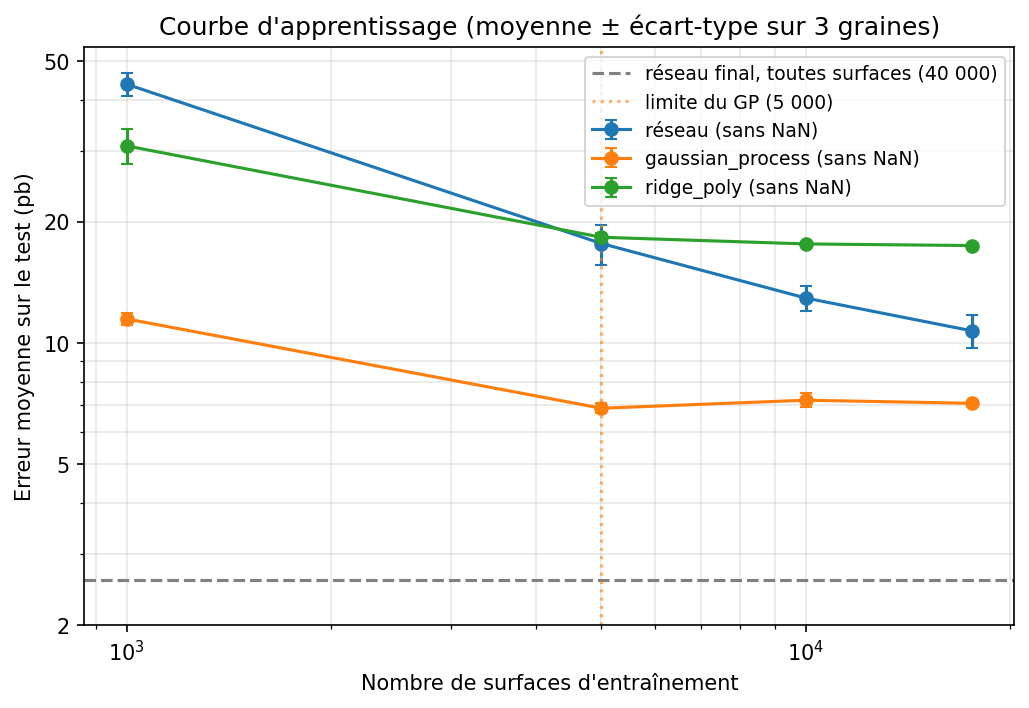
\includegraphics[width=0.75\textwidth]{etape3_courbe_apprentissage}
  \caption{Erreur moyenne sur le test selon le nombre de surfaces d'entraînement sans NaN (moyenne $\pm$
  écart-type sur 3 graines, échelles logarithmiques). Pointillés gris : réseau final entraîné sur les
  \num{40000} surfaces. Pointillés orange : limite de \num{5000} surfaces du GP.}
  \label{fig-ml-courbe}
\end{figure}

\begin{table}[H]
  \centering
  \caption{Erreur moyenne sur le test (pb, moyenne $\pm$ écart-type sur 3 graines) selon le nombre de surfaces
  d'entraînement.}
  \label{tab-ml-courbe}
  \small
  \begin{tabular}{rccc}
    \toprule
    Surfaces & Réseau & Processus gaussien & Ridge polynomiale \\
    \midrule
    \num{1000}  & $43{,}9 \pm 3{,}0$ & $11{,}5 \pm 0{,}4$ & $30{,}8 \pm 3{,}1$ \\
    \num{5000}  & $17{,}7 \pm 2{,}0$ & $6{,}89 \pm 0{,}19$ & $18{,}3 \pm 0{,}4$ \\
    \num{10000} & $12{,}9 \pm 1{,}0$ & $7{,}21 \pm 0{,}29$ & $17{,}6 \pm 0{,}1$ \\
    \num{17569} & $10{,}7 \pm 1{,}0$ & $7{,}09$ & $17{,}4$ \\
    \bottomrule
  \end{tabular}
\end{table}

Avec peu de données, le GP l'emporte nettement : \num{11.5}\pb\ avec \num{1000} surfaces, contre \num{43.9}\pb\
pour le réseau (\cref{fig-ml-courbe}, \cref{tab-ml-courbe}). La ridge plafonne autour de \num{17.5}\pb\ dès
\num{5000} surfaces : un polynôme de degré 4 ne peut pas faire mieux, quelle que soit la quantité de données. Le GP
plafonne à son tour à \num{5000} surfaces, à cause de sa limite de taille. Le réseau est le seul modèle dont
l'erreur baisse encore au bout de la courbe : \num{43.9}, puis \num{17.7}, \num{12.9} et \num{10.7}\pb. Sur les
\num{17569} surfaces, il ne rattrape pas le GP. Avec les \num{40000} surfaces, NaN compris, il descend à
\num{2.58}\pb.

\subsection{Bilan}
\label{sec-ml-bilan}

Sur un petit jeu de surfaces complètes, un processus gaussien est plus précis que notre réseau, pour un temps de
réponse qui passe encore le seuil. Le réseau prend l'avantage pour deux raisons. Son erreur continue de baisser
quand on ajoute des données, alors que le GP est limité par son coût et la ridge par sa forme. Et la perte masquée
lui permet d'apprendre sur toutes les surfaces, y compris les \SI{56}{\percent} qui ont un point manquant et qu'il
faut retirer pour les modèles classiques. Avec toutes les données, il fait \num{2.58}\pb\ sur le test, 2,7 fois
mieux que le GP, avec une erreur maximale de \num{93}\pb\ contre plus de \num{500}\pb\ pour tous les modèles
classiques, et il répond 5 à 6 fois plus vite.

Cette comparaison a ses limites. Les grilles d'hyperparamètres des modèles classiques sont petites, alors que le
réseau a été réglé en détail aux \cref{sec-architectures,sec-entrainement}. Nous n'avons pas essayé de compléter
les points manquants par imputation pour garder toutes les surfaces côté ML. Enfin, le coût du GP sur
\num{40000} surfaces est estimé à partir de sa complexité, pas mesuré.
